\documentclass[docid=PA09]{tcom_PA}
\begin{document}
\setcounter{section}{8}
\section{Preparation Activity 9 - Properties of CFLs}
{
\renewcommand{\thesubsubsection}{\thesubsection\alph{subsubsection}}
\subsection{Exercise 1}
\subsubsection{Item a}
\begin{alignat*}{2}
	S &\rightarrow aZbVc\mid T\mid U\\
	T &\rightarrow aZb\\
	U &\rightarrow bVc\\
	Z &\rightarrow aZb\mid \varepsilon \\
	V &\rightarrow bVc\mid \varepsilon
\end{alignat*}
Replace in $Z$.
\begin{alignat*}{2}
	S &\rightarrow aZbVc\mid T\mid U\\
	T &\rightarrow aZb\\
	U &\rightarrow bVc\\
	Z &\rightarrow T\mid \varepsilon \\
	V &\rightarrow bVc\mid \varepsilon
\end{alignat*}
Expand $T$ and $S$.
\begin{alignat*}{2}
	S &\rightarrow aTbVc\mid abVc\mid T\mid U\\
	T &\rightarrow ab\mid aTb\\
	U &\rightarrow bVc\\
	Z &\rightarrow T\mid \varepsilon \\
	V &\rightarrow bVc\mid \varepsilon
\end{alignat*}
Remove $Z$.
\begin{alignat*}{2}
	S &\rightarrow aTbVc\mid abVc\mid T\mid U\\
	T &\rightarrow ab\mid aTb\\
	U &\rightarrow bVc\\
	V &\rightarrow bVc\mid \varepsilon
\end{alignat*}
Replace in $V$.
\begin{alignat*}{2}
	S &\rightarrow aTbVc\mid abVc\mid T\mid U\\
	T &\rightarrow ab\mid aTb\\
	U &\rightarrow bVc\\
	V &\rightarrow U\mid \varepsilon
\end{alignat*}
Expand $U$ and $S$.
\begin{alignat*}{2}
	S &\rightarrow aTbUc\mid aTbc\mid abUc\mid abc\mid T\mid U\\
	T &\rightarrow ab\mid aTb\\
	U &\rightarrow bc\mid bUc\\
	V &\rightarrow U\mid \varepsilon
\end{alignat*}
Remove $V$.
\begin{alignat*}{2}
	S &\rightarrow aTbUc\mid aTbc\mid abUc\mid abc\mid T\mid U\\
	T &\rightarrow ab\mid aTb\\
	U &\rightarrow bc\mid bUc\\
\end{alignat*}
Replace symbols by generators.
\begin{alignat*}{2}
	S &\rightarrow ATBUC\mid ATBC\mid ABUC\mid ABC\mid T\mid U\\
	T &\rightarrow AB\mid ATB\\
	U &\rightarrow BC\mid BUC\\
	A &\rightarrow a\\
	B &\rightarrow b\\
	C &\rightarrow c
\end{alignat*}
Replace long expressions.
\begin{alignat*}{2}
	S   &\rightarrow AE_1\mid AE_4\mid AE_2\mid AE_5\mid T\mid U\\
	E_1 &\rightarrow TE_2\\
	E_2 &\rightarrow BE_3\\
	E_3 &\rightarrow UC\\
	E_4 &\rightarrow TE_5\\
	E_5 &\rightarrow BC\\
	E_6 &\rightarrow TB\\
	T   &\rightarrow AB\mid AE_6\\
	U   &\rightarrow BC\mid BE_3\\
	A   &\rightarrow a\\
	B   &\rightarrow b\\
	C   &\rightarrow c
\end{alignat*}
Replace $T$ and $U$ in $S$.
\begin{alignat*}{2}
	S   &\rightarrow AB\mid AE_1\mid AE_2\mid AE_4\mid AE_5\mid AE_6\mid BC\mid BE_3\\
	E_1 &\rightarrow TE_2\\
	E_2 &\rightarrow BE_3\\
	E_3 &\rightarrow UC\\
	E_4 &\rightarrow TE_5\\
	E_5 &\rightarrow BC\\
	E_6 &\rightarrow TB\\
	T   &\rightarrow AB\mid AE_6\\
	U   &\rightarrow BC\mid BE_3\\
	A   &\rightarrow a\\
	B   &\rightarrow b\\
	C   &\rightarrow c
\end{alignat*}
\subsubsection{Item b}
\begin{center}
	\begin{tikzpicture}
		\Tree 	[.$S$
					[.$A$
						$a$
					]
					[.$E_5$
						[.$B$
							$b$
						]
						[.$C$
							$c$
						]
					]
				]
	  \end{tikzpicture}
\end{center}
\subsubsection{Item c}
Consider a string $s=s_1s_2\ldots s_N$. $X_{i,j}$ is the set of variables that produce string $s[i:j]$.
\begin{alignat*}{2}
	X_{i,i} &= \{S\mid S \rightarrow s_i\}\\
	X_{i,j} &= \{S\mid \exists k \in [i,j] \colon \exists A\in X_{i,k},B\in X_{k+1,j}\colon S \rightarrow AB\}\;(j \geq i)
\end{alignat*}
\begin{center} \begin{tabular}{c || c | c | c}
	\backslashbox{$i$}{$j$} & $1             $ & $2             $ & $3      $ \\ \hline
	$1                    $ & $A             $ & $S, T          $ & $S      $ \\
    $2                    $ & \cellcolor{gray} & $B             $ & $S,E_5,U$ \\
	$3                    $ & \cellcolor{gray} & \cellcolor{gray} & $C      $ \\ \hline
	$                     $ & $a             $ & $b$     & $c$
\end{tabular} \end{center}
\subsection{Exercise 2}
\textcolor{red}{Incomplete.}
}
\end{document}
